\chapter{Introduction and Background}

The focus on reduction of greenhouse emissions from fossil fuels is today as important as ever. The rapid ongoing modifications of climate conditions are raising concerns and awareness in this regard. Total anthropogenic greenhouse emissions have continued to increase over 1970 to 2010, with larger absolute increase per decade toward the end of this period, with CO\textsubscript{2} emissions from fossil fuel combustion and industrial processes contributing about 78\% of the total. Annual anthropogenic GHG emissions have increased by 10 Gtons equivalent of CO2 between 2000 and 2010, with this increase directly coming from energy supply (47\%), industry (30\%), transport (11\%) and buildings (3\%) sectors \cite{IPCC2014}.

Global warming causes adverse effect and mutations on natural habitats and natural equilibriums of Earth, and is held responsible for increase of atmospheric temperature, acidification of oceans, melting of the permafrost, increased frequency of extreme weather events and others. As a result, many species struggle to adapt to these new environmental conditions and some are facing extinction. Even human related activities are in danger, as the natural habitat become more and more hostile to plants and animals. In the following sections the phenomenon will be explained in more details, and the role of transportation sector will be highlighted.

\section{Global warming and role of transport section emissions} \label{sec:global_warming}

\emph{Global warming} and \emph{Climate change} are terms used for describing the increase in surface and ocean temperature registered in the last century. Due to the accumulation of greenhouse gases, additional energy is stored in the atmosphere and the oceans, causing ice melting and warming of continents and atmosphere. 

\begin{figure}[h]
  \centering
  \includegraphics[width=0.8\textwidth]{figures/introduction/temp_rise.pdf}
  \caption{Global mean temperature estiamates based on land and ocean data\cite{GISS2016}}
  \label{antropogenic_ghg_emissions}
\end{figure}

Without additional efforts to reduce GHG emissions beyond those in place today, emissions growth is expected to persist driven by growth in global population and economic activities. Baseline scenarios, those without additional mitigation, result in global mean surface temperature increases in 2100 from \SI{3.7}{\celsius} to \SI{4.8}{\celsius} compared to pre-industrial levels \cite{IPCC2014}. Of the 49 Gt CO\textsubscript{2,eq} emitted in 2010, the \emph{transportation} sector is responsible for 14.3\% of the total, ranking as the fourth major emitter economic sector after Electricity and Heat production, Agriculture and Land use, and Industry.

\begin{figure}[h]
  \centering
\includegraphics[width=0.8\textwidth]{figures/introduction/antropogenic_ghg_emissions.pdf}
  \caption{Antropogenic GHG emissions by group of gases (1970 - 2010) \cite{IPCC2014}}
  \label{antropogenic_ghg_emissions}
\end{figure}

The scientific community mainly agrees on trying to keep the temperature increase with respect to pre-industrial levels under \SI{2}{\celsius}, equivalent to atmospheric concentrations in 2100 of about 450 ppm CO\textsubscript{2,eq}. The aforementioned scenarios include substantial cuts in anthropogenic GHG emissions by mid century through large scale changes in energy systems and potentially land use. Scenarios reaching these concentrations by 2100 are characterized by lower global GHG emissions in 2050 than in 2010, 40\% to 70\% lower globally, and emissions levels near zero Gt CO\textsubscript{2,eq} or below in 2100 \cite{IPCC2014}. In Figure \ref{fig:mitigationscenarios}, the reduction in emissions for the major economic sectors is reported. It's possible to notice how, especially in the case without heavy implementation of carbon dioxide capture plants, the amount of greenhouse gases released in the atmosphere by transport must be greatly reduced.

\begin{figure}[ht]
  \centering
  \includegraphics[width=\textwidth]{figures/introduction/mitigation_scenarios.pdf}
  \caption{Review of different mitigation scenarios for 450 ppm \label{fig:mitigationscenarios}}
\end{figure}

The chart represents a review of the major models and scenarios available to date, and taken into consideration in \cite{IPCC2014}. According to the same study, efficiency enhancements and behavioural changes aimed at reducing energy demand compared to baseline scenarios without compromising development, are a key mitigation strategy in scenarios reaching atmospheric CO\textsubscript{2,eq} concentrations of about 450 to about 500 ppm by 2100.

The transport sector accounted for 27\% of final energy use and 6.7 Gt CO\textsubscript{2} direct emissions in 2010, with baseline CO\textsubscript{2} emissions projected to approximately double by 2050. Technical and behavioural mitigation measures for all transport modes, plus new infrastructure and urban redevelopment investments, could reduce final energy demand in 2050 by around 40\% below the baseline \cite{IPCC2014}.

A study by Unger and al.~\cite{Unger2010} attributes a radiative forcing value to different economic sectors that are the main emitters in today economy. The radiative forcing concept has been developed in order to quantify the human and natural influence on the climate system, and is defined as the net energy flux difference at the top of the atmosphere. In Figure~\ref{fig:radiative_forcing}, the positive and negative contributions of the different economic sectors are presented. It's important to notice how on-road transportation is foreseen to be the major responsible for increasing of atmospheric energy content in 2020, and the second most important factor in 2100. This is due to the peculiar composition of exhaust gases produced by vehicles: the production is  mainly constituted by components that contribute to trapping heat. Other sectors, as the power sector, produce much more components that trap heat, but the net contribution is reduced by the amount of components as black-carbon, that reflects the solar radiation and contribute to cooling down the atmosphere. 

\begin{figure}[ht]
  \centering
  \includegraphics[width=\textwidth]{figures/introduction/radiative_forcing.png}
  \caption{Radiative forcing due to 2000 level emissions grouped by sector in a) 2020 and b) 2100 \label{fig:radiative_forcing}}
\end{figure}

\section{Current transportation scenario}

The average efficiency of modern internal combustion engines is measured to be around 32\% - 36\% for Diesel engines, and around 29\% - 32\% for Gasoline engines.

According to the evidence reported in section~\ref{sec:global_warming}, being the transportation sector one of the main culprits for global warming, an increase in efficiency of passenger vehicles can play an important role in mitigating climate change. Figure~\ref{fig:average_fuel_efficiency} shows how, in the 1980 - 2014 considered timeframe, the specific fuel consumption of U.S. vehicles has been reduced thanks to technical advancements~\cite{BureauofTransportationStatistics2016}.

\begin{figure}[ht]
  \centering
  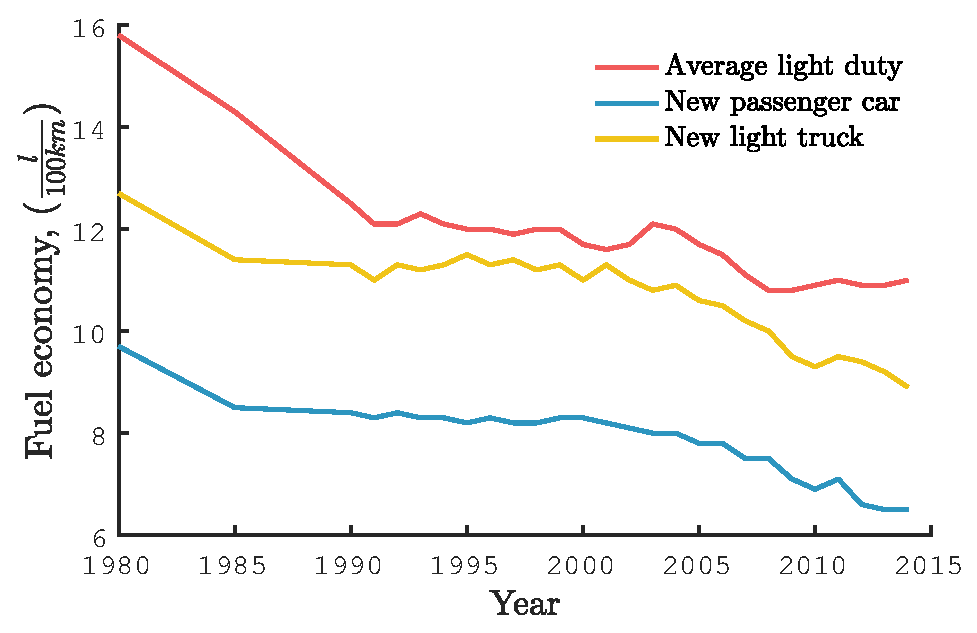
\includegraphics[width=0.8\textwidth]{figures/introduction/average_fuel_efficiency.eps}
  \caption{Average fuel efficiency for U.S. vehicles \label{fig:average_fuel_efficiency} }
\end{figure}

Taking a more in depth look at the emissions figure of the transportation economy itself, when considering the energy use by transportation mode in 2013, Highwway is by far the sector that consumes the greater share of the total (83.2\%), followed by Air transportation (6.9\%) and Water transportation (3.9\%). The Highway energy usage can be once again split between Light-duty (52.2\%), Combination Truck (15.3\%), Single-unit truck (7.6\%), and Bus (1.1\%). Certified air carriers experienced the largest total decrease in fuel consumption, consuming about 3.6 billion fewer gallons of jet fuel in 2014 than in 2000. General aviation gasoline showed the largest percent decrease in fuel consumption from 2000 to 2014, declining by 40.8 percent. Additionally, water modes powered by residual fuel oil also showed a large decrease, declining by nearly 2.6 billion gallons during the same period. Consistent with increases in vehicle-miles traveled, light-duty highway vehicles used about 430 million more gallons of gasoline in 2014 than in 2000~\cite{BureauofTransportationStatistics2016a}.

According to the evidence shown, the amount of effort spent on researching and experimenting new and more advanced ways of reducing transportation energy consumption is justified. Numerous different technical trends are nowadays gaining traction in the automotive field, such as downsizing and turbocharging of gasoline engines, or the usage of different cycles. A more in depth analysis will be provided in Section~\ref{sec:technology_improvements}.

\section{Evolution in internal combustion engines technology and efficiency}

In this section a review of the key technical improvements occurred to internal combustion engines in the last decades is presented, among with a brief explanation of the current emission limitation rules for both the USA and Europe. The final section will cover the importance of \emph{Waste Heat Recovery} (WHR) and why it needs to be researched and adopted in the next years in order to achieve the planned emissions limitation objectives.

\subsection{Improvements on overall engine efficiency in the last decades}

Since the petroleum crysis of the '70s, an increasing effort on reduction of fuel consumption and increase of power density has begun.

\begin{figure}[ht]
  \centering
  \includegraphics[width=\textwidth]{figures/review/adj_fuel_economy.pdf}
  \caption{Adjusted CO\textsubscript{2} and fuel economy for vehicles model year from 1975 to 2016\label{fig:adj_fuel_economy} }
\end{figure}

As shown in Figure~\ref{fig:adj_fuel_economy}~\cite{EPA2016}, during the last four decades, the fuel consumption and carbon dioxide emissions has been vastly reduced. This great improvement has been possible thanks to some key technical turning points.

One of the main design aspects that have changed significantly over time is how the fuel is delivered into the engine. Until the early 1980s the majority of engines used carburetors to meter fuel delivered to the combustion chamber. More recently, engines with gasoline direct injection (GDI) have begun to replace engines with port fuel injection. GDI equipped engines were first introduced with very limited production in Model Year (MY) 2007. Eight years later GDI engines were installed in about 42\% of MY 2015 vehicles, and are projected to achieve a 49\% market share in MY 2016~\cite{EPA2016}.

Another key aspect of engine design that has been vastly improved is the valve-train. The number of valves per cylinder and the ability to alter valve timing during the combustion cycle allowed significant power and efficiency improvements, as nowadays almost the entire fleet of the most relevant car manufacturers has converted to multi-valve design. While some three and five valve engines have been produced, the vast majority of multi-valve engines are based on four valves per cylinder~\cite{EPA2016}. In addition to the number of valves per cylinder, designs have evolved that allow engine valves to vary the timing when they are opened or closed with respect to the combustion cycle, creating more flexibility to control engine efficiency, power, and emissions. In Figure~\ref{fig:improvement_valve_fuel_delivery}, the fuel consumption reduction made possible by the improved valve-train and fuel delivery is shown. 

\begin{figure}[ht]
  \centering
  \includegraphics[width=0.7\textwidth]{figures/review/improvement_valve_fuel_delivery.pdf}
  \caption{Trends of fuel consumption variation with the introduction of major fuel delivery and valve-train control technologies \label{fig:improvement_valve_fuel_delivery} }
\end{figure}

As a result of the new fuel delivery systems, along with other reasons, two very noticeable trends in horsepower and displacement delineated. Average horsepower climbed consistently from MY 1982 to MY 2008. Since MY 2008, horsepower trends have been less consistent, and may be beginning to flatten out. From MY 1975 to 1987, the average engine displacement of new vehicles dropped dramatically by nearly 40 \%. From MY 1988 to 2004, displacement generally grew slowly, but the trend reversed in 2005 and engine displacement has been generally decreasing since. In MY 2016, engine displacement is projected to reach the lowest point on record, below the previous lowest average displacement reached in MY 1987~\cite{EPA2016}.

The contrasting trends in horsepower increase and displacement decrease are a proof of the continued improvements in engine design and of the impact of new technologies. The final result is a steady quasi-linear increase of the power density from around 0.5~$\frac{HP}{Displacement}$ in 1975 to around 1.4~$\frac{HP}{Displacement}$ in 2016, with a growth rate of 0.02~$\frac{HP}{in^{2} \cdot year}$. Also the average number of cylinders has gradually reduced.

In Figure~\ref{fig:technology_trends}, a summary of the time trends of the major innovations is reported.

\begin{figure}[ht]
  \centering  \includegraphics[width=\textwidth]{figures/review/technology_trends.png}
  \caption{Percentage of MY equipped with a certain technology  \label{fig:technology_trends} }
\end{figure}


\subsection{Emission limitations and trends in nowadays technology improvement}
\label{sec:technology_improvements}

Emission limitations are among the main drivers that fostered the continuous strive of greater efficiency in internal combustion engines. In Figure~\ref{fig:emission_standards} a review of the most important emissions standards from across the world, and their Euro equivalence is presented~\cite{Miller2014}. In Figure~\ref{fig:emission_levels} are reported the emission limits for gasoline and diesel powered light vehicles in both USA and Europe~\cite{Transportpolicy.net2016}.

\begin{figure}[ht]
  \centering
  \includegraphics[width=\textwidth]{figures/review/emission_standards.png}
  \caption{Comparison of emissions standards with reference to Euro standards\label{fig:emission_standards} }
\end{figure}

\begin{figure}[ht]
  \centering
  \includegraphics[width=\textwidth]{figures/review/emissions_levels.png}
  \caption{Emissions limits for a) Gasoline and b) Diesel light vehicles in USA and Europe\label{fig:emission_levels} }
\end{figure}

In order to respect the emission standards imposed by current and future rules, the major car manufacturers are adopting new technologies, and some trends are delineating. 

Probably the most noticeable trend in new engines is the \emph{turbo-downsizing}. This new group of engines is characterized usually by a similar power output with respect to the engine that are replacing, but a smaller displacement. This result is achieved by the introduction of turbochargers and, often but not always, GDI. Turbo downsized engines are an approach to engine design that provides increased fuel economy by using a smaller engine for most vehicle operation, while retaining the ability to provide more power via the turbocharger, when needed. Turbocharged engines are projected to constitute 22\% of new vehicle production in 2016, and the penetration trend appears to increase rapidly~\cite{EPA2016}. This is due to the fact the traditionally turbocharged engines were mainly used in high performance vehicles, while now they are being used also on mainstream vehicles. The increased power density and torque made available by the adoption of the turbocharger allows the shifting to designs with fewer cylinders, while the combination with GDI allows a more efficient engine operation and increases the resistance to knocking. In MY 2016, more than 90\% of new vehicles with gasoline turbocharged engines also use GDI~\cite{EPA2016}. In Figure~\ref{fig:turbodownsizing_distribution}, the distribution of gasoline turbo vehicles is shown. Other new technologies that are gaining traction in the engine design environment are Cylinder Deactivation, Non-Hybrid Stop/Start, and more advanced transmissions, both in form of transmissions with seven or more gears or Continuous-Variable Transmissions (CVT).

\begin{figure}[ht]
  \centering
  \includegraphics[width=0.8\textwidth]{figures/review/turbodownsizing_distribution.pdf}
  \caption{Distribution of Gasoline Turbo Vehicles by Displacement and Horsepower, MY 2010, 2013, and 2016\label{fig:turbodownsizing_distribution} }
\end{figure}



\emph{Hybrid} vehicle technology is the most diffused technique used to increase the fuel efficiency in ways that transcend the pure ICE efficiency increase. Hybrid vehicles utilize larger battery packs, electric motors, and other components that can  increase vehicle fuel economy. Benefits of hybrids include:
\begin{itemize}
\item regenerative braking which can capture energy that is otherwise lost in conventional friction braking to charge the battery
\item availability of two sources of on-board power which can allow the engine to be operated at or  near its peak efficiency more often
\item shutting off the engine at idle.
\end{itemize} 

Most hybrids provide higher fuel economy than comparable vehicles, although some hybrids have been offered as more performance-oriented vehicles with more minor fuel economy improvements. In Figure~\ref{fig:hybrids} it's shown the distribution in time of the fuel economy between hybrid and non hybrid vehicles, and the historical production of hybrid and electric vehicles.

\begin{figure}[ht]
  \centering
  \includegraphics[width=\textwidth]{figures/review/hybrid.png}
  \caption{Comparison fuel economy between non hybrid and hybrid cars and hybrid cars production \label{fig:hybrids} }
\end{figure}


While the average fuel economy of hybrid cars remains higher than the average fuel economy  of non-hybrid cars, the difference appears to be narrowing. Average hybrid car fuel economy  has been relatively stable since MY 2001, while the fuel economy of the average non-hybrid car has increased more than 27\%. Since MY 2004, the difference in fuel economy between the average hybrid midsize car and the average non-hybrid midsize gasoline car has narrowed from about 25 mpg to about 14 mpg. The primary reason for this trend is continued improvements to the internal combustion engine. Additionally, many technologies introduced or emphasized in early hybrids, such as improved aerodynamics, low rolling resistance tires, and increased use of lightweight materials, have also become more common on non-hybrid vehicles~\cite{EPA2016}.

\subsection{The importance of waste heat recovery}

In the previous sections a brief review of how some of the key technical improvements have modified engine design, performances and fuel consumption have been provided.

One of the main causes of the relatively low efficiency of even modern ICEs is that a significant amount of energy produced by fuel combustion is wasted in form of heat, then not used to produce useful power. In internal combustion engines, only a small part of the fuel energy flow is transformed into power available at the crankshaft. For the best points of operation, diesel engines have a maximum efficiency approaching 45\% while gasoline engines have efficiencies of about 35\%. For both engines, the most part of the fuel energy flow is therefore lost as coolant heat flow and exhaust gases heat flow. In everyday operating conditions, cars have average engine efficiencies on driving cycles well below their top values, with the heat flow lost in the exhaust gases and the engine coolant increasing accordingly. In many driving conditions, the waste heat flow represents an important part of the fuel energy flow. The energy flow potentially available to be converted to usable power in the exhaust gases and the coolant is therefore quite significant~\cite{Boretti2012}. Considering the large number of vehicles in the world, such waste energy makes great impact to our environment globally.

\begin{figure}[ht]
  \centering
  \includegraphics[width=0.6\textwidth]{figures/review/sankey.png}
  \caption{Typical energy balance of a Euro 6 diesel engine\label{fig:sankey_energy} }
\end{figure}
~

It has been estimated that the thermal efficiency of a modern IC engine is limited to 20 - 40\% while 33\% of the fuel energy from a typical medium-size passenger vehicle is carried away by exhaust gases and 29\% is carried away by engine cooling water in urban traffic conditions. Depending on engine type and operating conditions, the IC exhaust gas temperature usually varies from 500 to \SI{900}{\celsius} and engine cooling water temperature is around \SI{100}{\celsius}. It is reported that for a typical light duty 4 cylinder spark ignition engine, the waste energy carried by the exhaust gas ranges from 4.6 to 120 kW and cooling water heat ranges from 9 to 48 kW \cite{ElChammas2005}, which makes the exhaust gas and engine cooling heat very attractive for energy recovery. It's possible to harvest part of this waste energy from vehicles and produce regenerated mechanical or electrical power.

According to \cite{Conklin2010}, experimental data coming from a series of tests on a turbo-charged 2007 Saab vehicle shows engine-out exhaust temperature from 400 to \SI{600}{\celsius}. The exhaust temperature range of naturally aspirated gasoline engine is higher, typically from 450 to \SI{800}{\celsius}. The same research performed a FTP-75 test cycle with the aforementioned vehicle, and measured that the total fuel energy consumed during the course of the driving cycle is approximately 58.5 MJ, or about 1.7 L of unleaded gasoline fuel. The percentage of fuel energy converted to useful work for this driving cycle (i.e. the vehicle thermal efficiency) is 10.4\%. A much larger portion of fuel energy, 27.7\%, exits the vehicle in the form of thermal energy in the exhaust, while the remaining 61.9\% of the energy balance consists of energy losses to friction, coolant, and other. Only a portion of the energy in the exhaust is available for recovery due to process irreversibilities, ambient conditions, or other.

% BEGIN RECEIVE ORGTBL first_second_law
\begin{table}
  \begin{center}
    \begin{tabular}{lrr}
      & 1st law & 2nd law \\
      \hline
      Brake work & 10.4\% & 9.7\% \\
      Exhaust & 27.7\% & 8.4\% \\
      Irreversibilities, Friction, Coolant, and other & 61.9\% & 81.9\% \\
    \end{tabular}
    % % END RECEIVE ORGTBL first_second_law
    % \begin{comment}
    %   #+ORGTBL: SEND first_second_law orgtbl-to-latex
    %   |                                                 | 1st law | 2nd law |
    %   |-------------------------------------------------+---------+---------|
    %   | Brake work                                      |   10.4% |    9.7% |
    %   | Exhaust                                         |   27.7% |    8.4% |
    %   | Irreversibilities, Friction, Coolant, and other |   61.9% |   81.9% |
    % \end{comment}
    \caption{1\textsuperscript{st} and 2\textsuperscript{nd} law of thermodynamics fuel energy and exergy distributions}
    \label{table:1st_2nd_law}
  \end{center}
\end{table}

In Table~\ref{table:1st_2nd_law} are reported the energy and exergy distributions with respect of the fuel entering the engine. It's possible to notice how, according to the 2\textsuperscript{nd} law of thermodynamics, the exhaust exergy is nearly as high as the amount of brake work. Thus, there is an abundant amount of available energy present in the exhaust of modern gasoline vehicles that can be used to improve overall system efficiency if an effective means of energy recovery can be employed. In another research \cite{Dolz2012}  the value of exhaust gases mentioned to be 18.6\% of total combustion energy. It is also found that by installing heat exchanger to recover exhaust energy of the engine could be saved up to 34\% of fuel saving \cite{Wang2013}.

Many studies highlighted the validity of the idea of recovering this waste heat to produce additional power, and the research and actual production efforts showed promising results. In Table~\ref{Table:ORC_research_list} are listed some of the most relevant research and production vehicles equipped with a waste heat recovery system, among with the achieved increase in thermal and mechanical efficiency.

\begin{table}[]
  \centering
  \resizebox{\textwidth}{!}{
    \begin{tabular}{lllllll}
      \hline
      Reference                        & Year & Vehicle       & Heat Source                 & Research method & $\Delta\eta_{th}$ & $\Delta\eta_{mec}$ \\ \hline
      \cite{Oomori1993b}               & 1993 & Passenger car & Coolant                     & Experiment      & /                 & 3\%                \\
      \cite{ElChammas2005}             & 2005 & HEV           & Exhaust                     & Numerical       & 1.3-5\%           & /                  \\
      \cite{Arias2006}                 & 2006 & Prius         & Exhaust + engine block      & Numerical       & 5.50\%            & /                  \\
      \cite{Endo2007, Kadota2008}      & 2007 & HEV           & Exhaust                     & Experiment      & 3.80\%            & /                  \\
      \cite{Freymann2008}              & 2008 & 3 series      & Exhaust + Coolant           & Experiment      & 5.70\%            & /                  \\
      \cite{Duparchy2009}              & 2009 & HEV-Prius     & Exhaust + Coolant           & Numerical       & /                 & 9\%                \\
      \cite{He2011, ZHANG2011}         & 2011 & Toyota 8A-FE  & Exhaust, Lubricant, Coolant & Experiment      & 12-17.3\%         & /                  \\
      \cite{Freymann2012, Horsta}      & 2012 & 5 series      & Exhaust                     & Experiment      & /                 & 6\%                \\
      \cite{Boretti2012, Boretti2012a} & 2012 & 1.8L engine   & Exhaust + Coolant           & Numerical       & 1.7-5.1\%         & /                  \\
      \cite{Wang2016a}                 & 2012 & BL18T engine  & Exhaust + Coolant           & Numerical       & 3-6\%             & /                  \\
      \cite{Domingues2012}             & 2013 & 2.8L VR6      & Exhaust                     & Experiment      & /                 & 2.64-6.96\%        \\ \hline
    \end{tabular}}
  \caption{Research results on waste heat recovery benefits}
  \label{Table:ORC_research_list}
\end{table}

\section{Objectives and structure of the thesis}

The main objective of the thesis is to compare three different technologies that aim at recovering waste heat produced by the internal combustion engine. In particular, two different \emph{Organic Rankine} bottoming \emph{Cycles} (ORC) paired with an Otto-cycle engine, and a \emph{Split-Cycle Engine} with \emph{isothermal compression} and \emph{integrated waste heat recovery}.

The comparison will be performed via MATLAB/Simulink simulations. A backward-looking model will take as input the velocity profile of a driving cycle for which experimental data is available, then the torque and angular speed at the engine will be calculated through a simulated transmission. Furthermore, engine maps will be extracted from experimental data along with characteristics and performances of the heat exchangers, making possible the calculation of flow rate, temperature and heat flux for both the exhaust gases and the coolant. Once the waste heat data will be available, the bottoming cycle model will be introduced. Starting from the output of the powertrain model, the recovered energy and produced power will be calculated.

\emph{ADD METHODOLOGIES MODEL SPLIT-CYCLE}

\emph{TO BE CONTINUED WITH STRUCTURE}


%%% Local Variables:
%%% mode: latex
%%% TeX-engine: xetex
%%% TeX-master: "thesis"
%%% End:
%%% \end{document}
